% =========================================================================
% RESULTS
% =========================================================================
\section{Results}
In this section the results of the measurements with the specified conditions are presented. The measurements were performed with a fixed timeout of 1000 ms.

\subsection{Normal Operation}
These are the results of the measurements with normal operation. Normal operation means that the master node and the slave node are connected to the same network and there is no heavy CPU load. These measurements were performed to fulfill the requirements R-RT07. 

\begin{figure}[H]
\centering
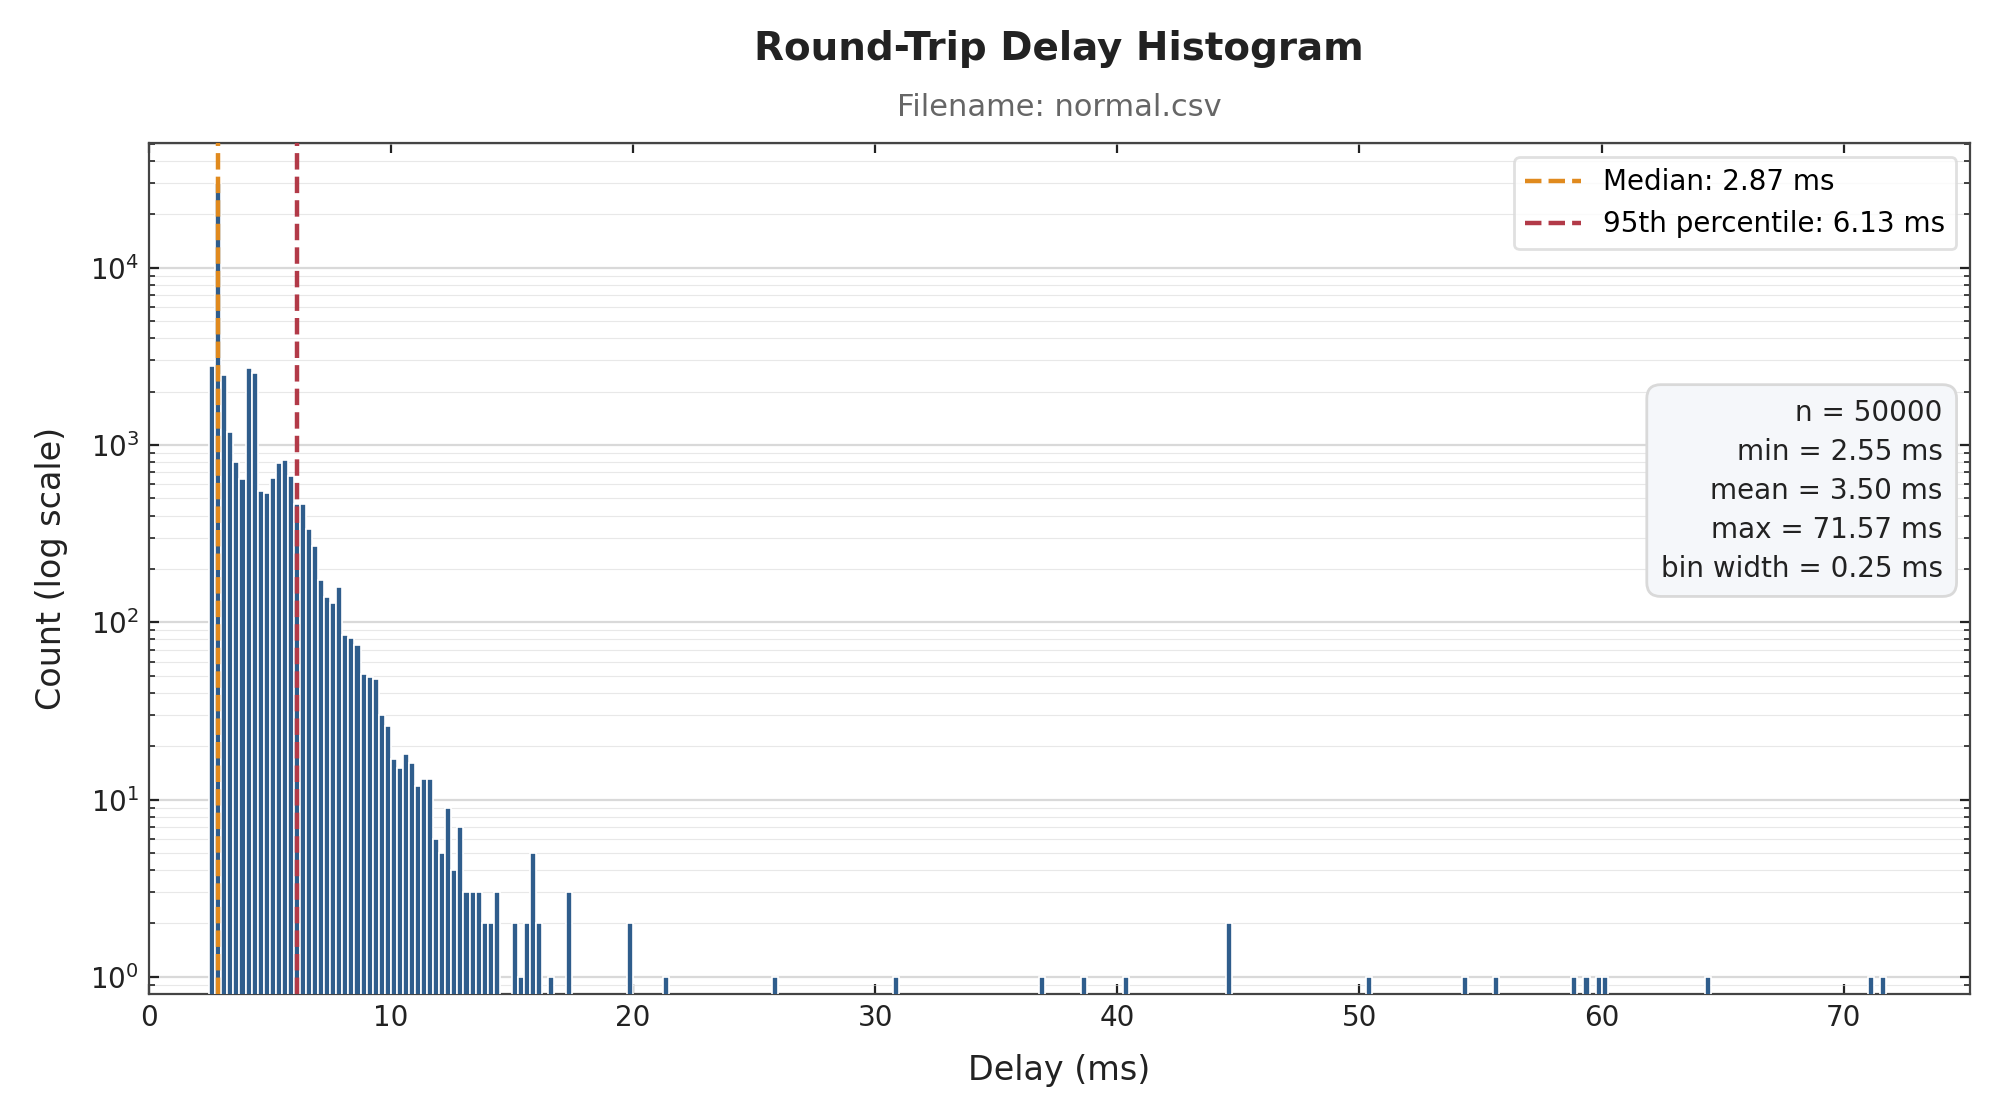
\includegraphics[width=0.75\textwidth]{./../results/normal.png}
\caption{Measurement results for 50000 measurements under normal conditions.}
\end{figure}

\subsection{High Network Load}
These are the results of the measurements with high network load. To simulate a high network load the tool \texttt{iperf} was used in combination with another client which was a notebook connected to the same network. These measurements were performed to fulfill the requirements R-RT08.

\begin{figure}[H]
\centering
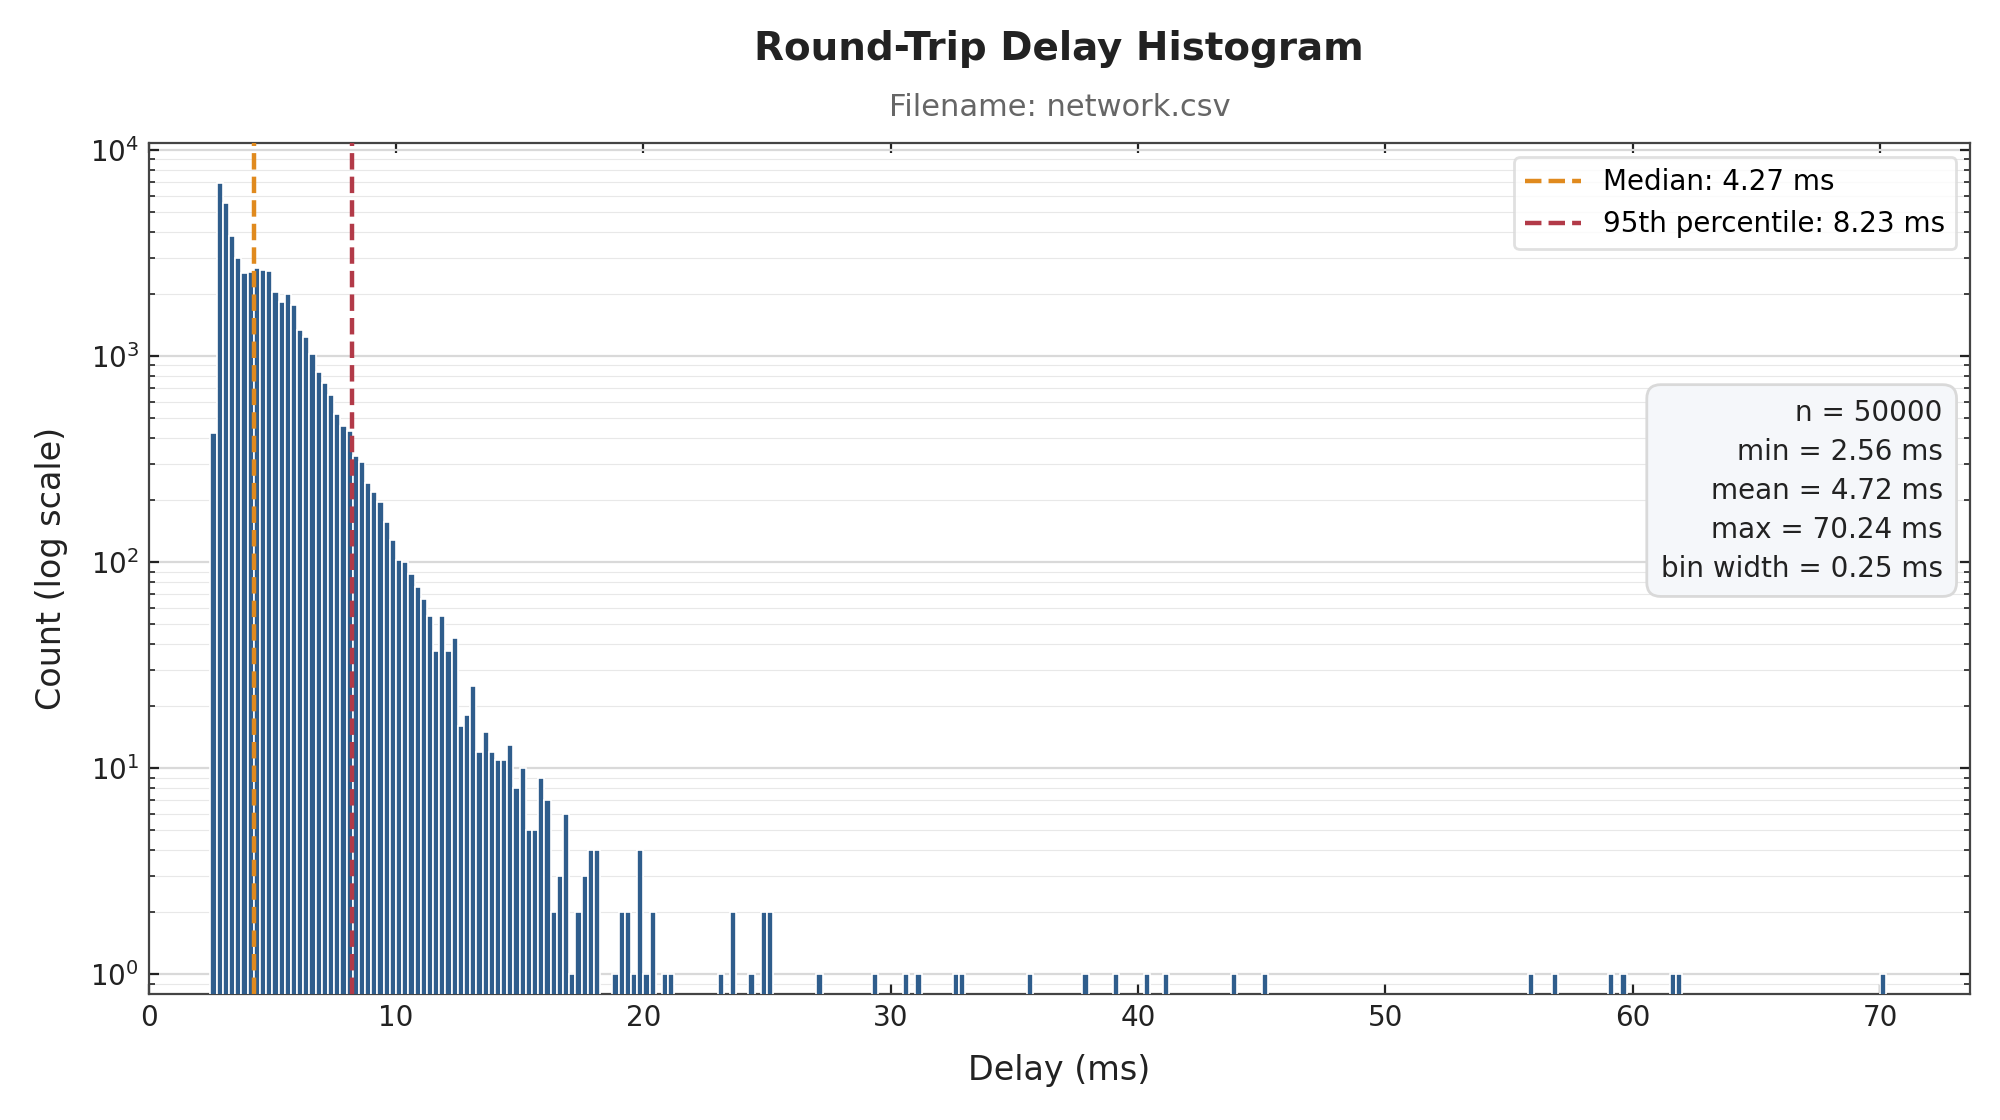
\includegraphics[width=0.75\textwidth]{./../results/network.png}
\caption{Measurement results for 50000 measurements under high network load.}
\end{figure}

\subsection{High CPU Load}
These are the results of the measurements with high network load. To simulate a high network load the tool \texttt{prime95} was used. This tool calculates prime numbers to generate load on the CPU. The tool was run on the master node. These measurements were performed to fulfill the requirements R-RT09.

\begin{figure}[H]
\centering
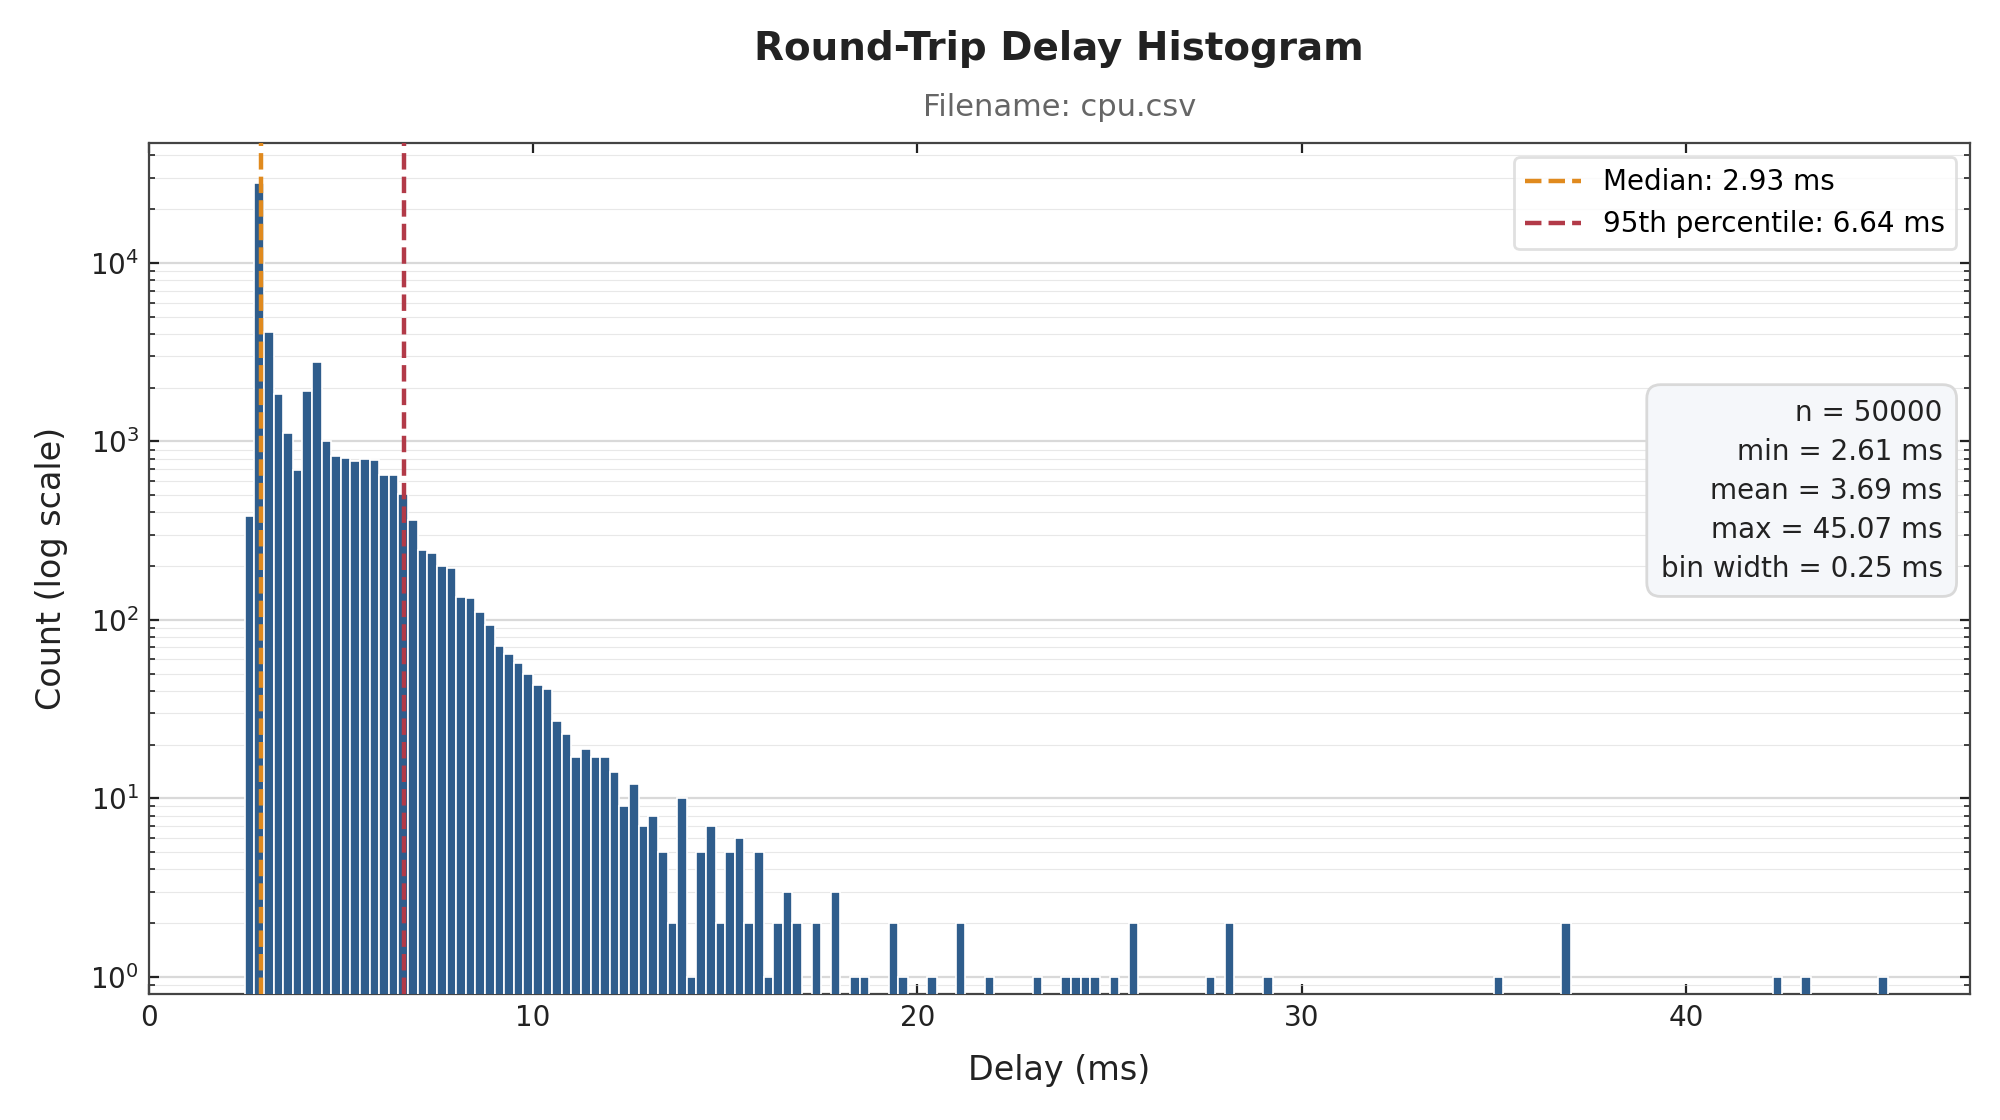
\includegraphics[width=0.75\textwidth]{./../results/cpu.png}
\caption{Measurement results for 50000 measurements under CPU load.}
\end{figure}

\subsection{Overview Tables}

\subsubsection{Statistics}
% Generated by Analyse_RTT.py - do not edit manually.
% Requires tabularray and the colours rowlight, rowdark, techred.
\begin{longtblr}[caption = {Round-trip delay statistics}, label = {tab:rtt-statistics}]{
  width = \textwidth,
  colspec = {Q[l,m,font=\bfseries] X[c,m] X[c,m] X[c,m] X[c,m] X[c,m]},
  rowhead = 1,
  row{even} = {bg=rowlight},
  row{odd} = {bg=rowdark},
  row{1} = {bg=techred, fg=white, font=\bfseries},
}
  Data set & Min [ms] & Mean [ms] & Median [ms] & p95 [ms] & Max [ms] \\
  normal & 2.550 & 3.497 & 2.870 & 6.132 & 71.566 \\
  cpu & 2.608 & 3.695 & 2.928 & 6.640 & 45.066 \\
  network & 2.563 & 4.721 & 4.271 & 8.227 & 70.245 \\
\end{longtblr}


\subsubsection{Completeness}
% Generated by Analyse_RTT.py - do not edit manually.
% Requires tabularray and the colours rowlight, rowdark, techred.
\begin{longtblr}[caption = {Round-trip measurement completeness}, label = {tab:rtt-completeness}]{
  width = \textwidth,
  colspec = {Q[l,m,font=\bfseries] X[c,m] X[c,m] X[c,m] X[c,m] X[c,m]},
  rowhead = 1,
  row{even} = {bg=rowlight},
  row{odd} = {bg=rowdark},
  row{1} = {bg=techred, fg=white, font=\bfseries},
}
  Data set & Sent & Received & Timeouts & Aborted & No valid response \\
  normal & 50000 & 50000 & 0 & 0 & 0/50000 (0.00\,\%) \\
  cpu & 50000 & 50000 & 0 & 0 & 0/50000 (0.00\,\%) \\
  network & 50708 & 50000 & 708 & 0 & 708/50708 (1.40\,\%) \\
\end{longtblr}
